\documentclass[../main.tex]{subfiles}

\begin{document}

\subsection{Web Application Development and Evaluation}

Aim 3 will focus on the development of an interactive web application, LeafAI, capable of generating and executing user queries. 

\subsubsection{Application Design}

LeafAI will be developed using a 3-tier architecture similiar to Leaf \cite{dobbins2019leaf}: a back-end with clinical and application databases, and server hosting an API (discussed in Aim 2), and a front-end web application. The key innovation of the web application will be its primary user interface, a chat-like design we expect will be familiar to most users of applications such as Microsoft Teams or Slack.

A chat-like interface for cohort discovery is both novel and a logical design choice given the natural language interface of LeafAI. An example of LeafAI's proposed chat interface is shown in \ref{aim3_fig_demo}. 

\begin{figure}[h!]
  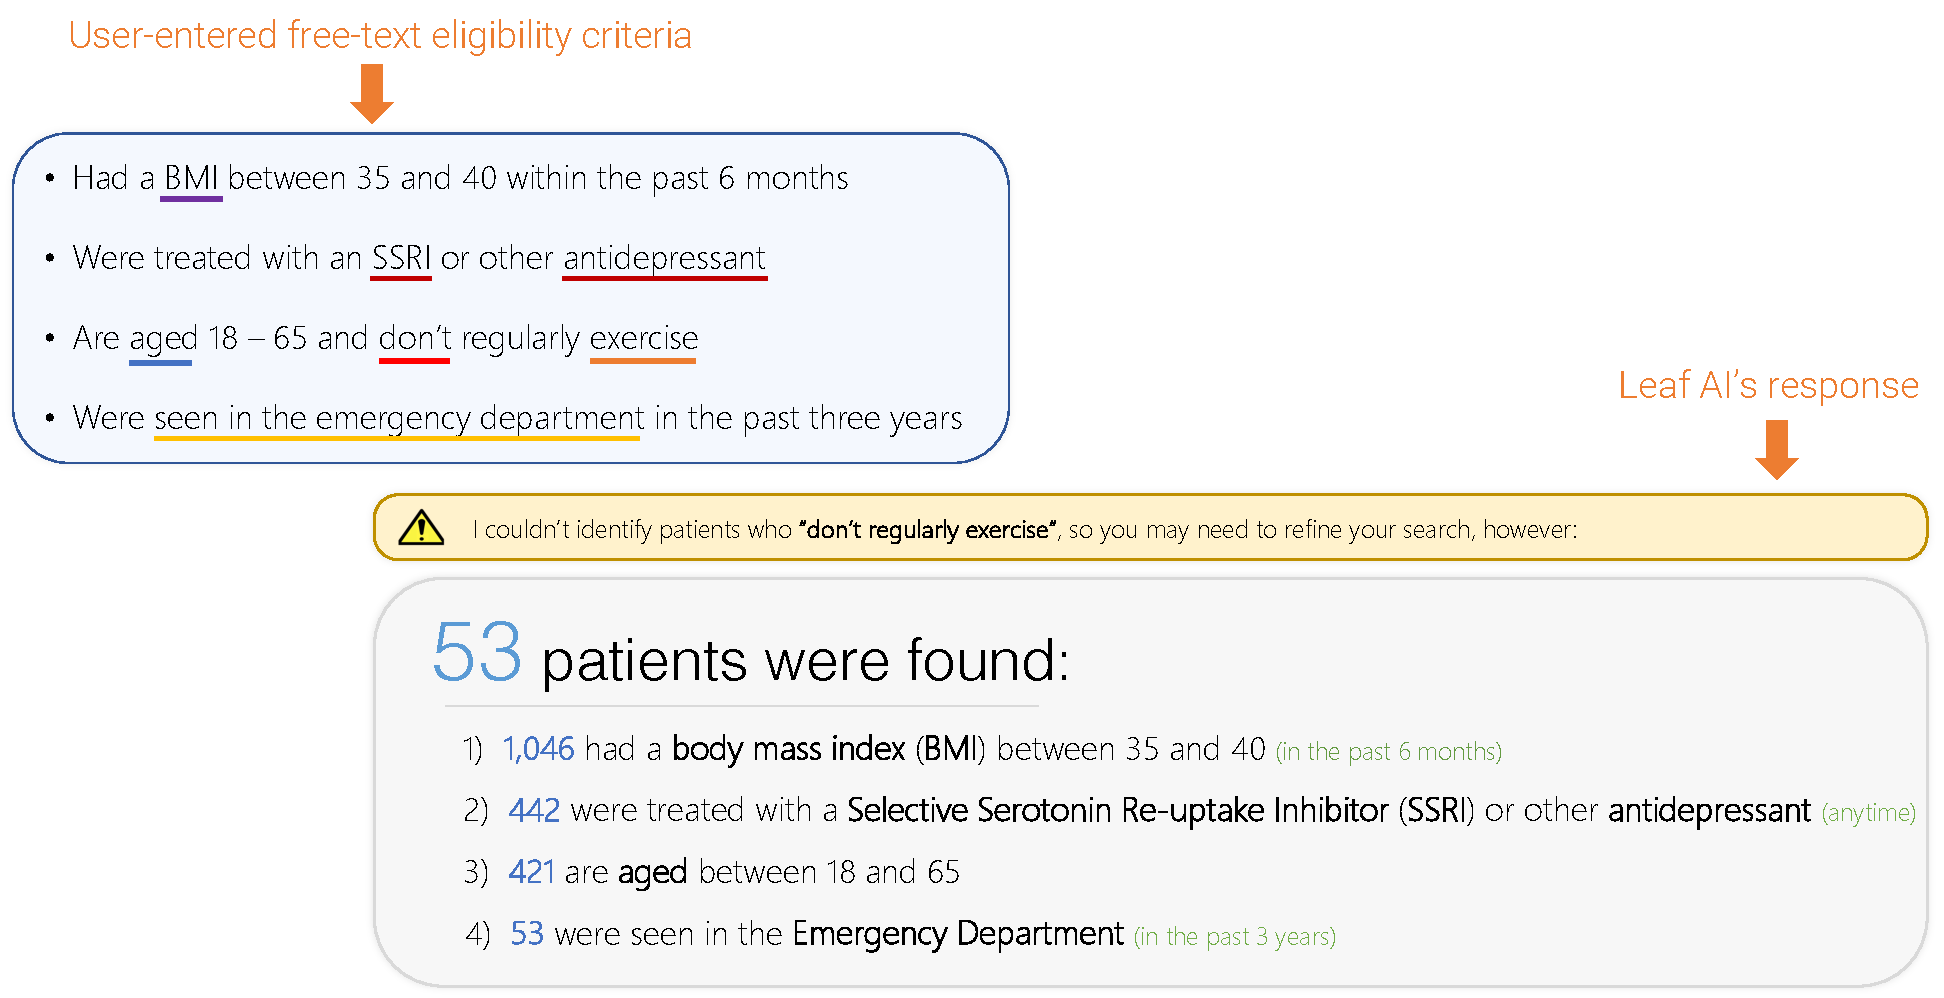
\includegraphics[scale=0.58]{Figures/Aim3/aim3_demo.pdf}  
  \caption{}
\label{aim3_fig_demo}
\end{figure}

Cohort discovery is a form of data exploration. As Derthick and Roth write, "...the data exploration process is not characterized by monotonic progress towards a goal, but rather involves much backtracking and opportunistic goal revision" \cite{derthick2001enhancing}. Put another way, user goals and perceptions may change over the course of their exploration. With ubiquitous vertical scrolling - where more recent actions and utterances are inserted downward while history is preserved upward - chat-like user interfaces facilitate user understanding of past utterances and actions. Persisted, easily viewable history of user utterances and actions facilitates what Gergle \textit{et al} call "conversational grounding" \cite{gergle2004persistence}, that is, accessible data to guide users to acquired findings and information.

% IMMEDIATE FEEDBACK WHILE TYPING
\begin{figure}[h!]
  \centering
  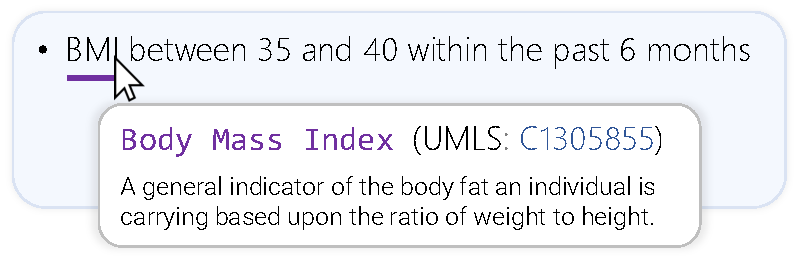
\includegraphics[scale=1]{Figures/Aim3/aim3_mouse_hover.pdf}  
  \caption{}
\label{aim3_fig_mouse_hover}
\end{figure}

% ITERATION
Data exploration is thus iterative; users explore, try, and learn over the course of multiple attempts.

\begin{figure}[h!]
  \centering
  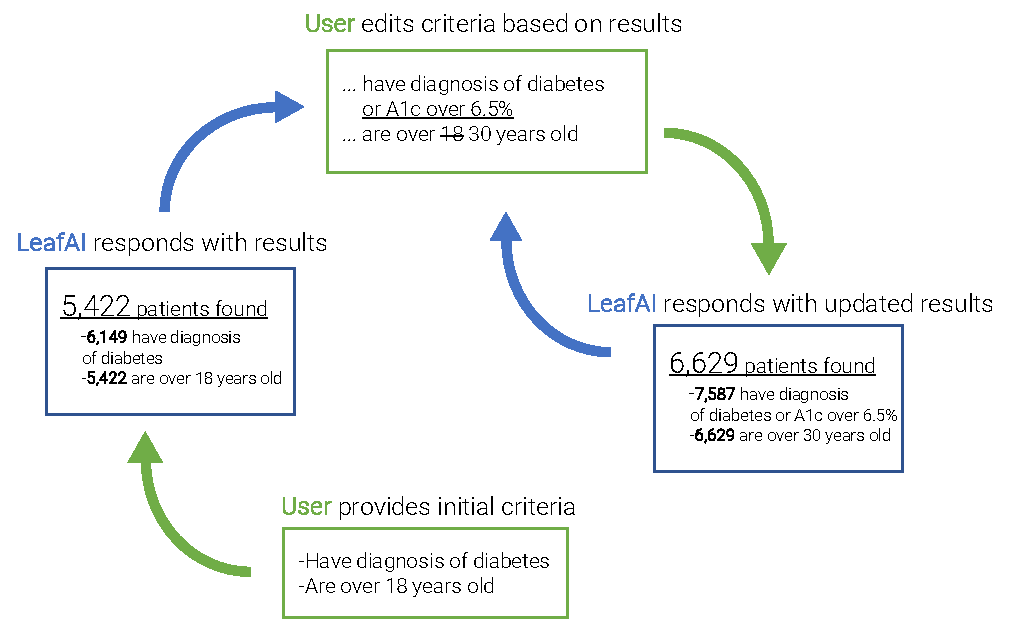
\includegraphics[scale=1]{Figures/Aim3/aim3_feedback_loop.pdf}  
  \caption{}
\label{aim3_fig_feedback_loop}
\end{figure}

% IMMEDIATE FEEDBACK WHILE WAITING
% cite: https://academic.oup.com/iwc/article/31/1/1/5369675
\begin{figure}[h!]
  \centering
  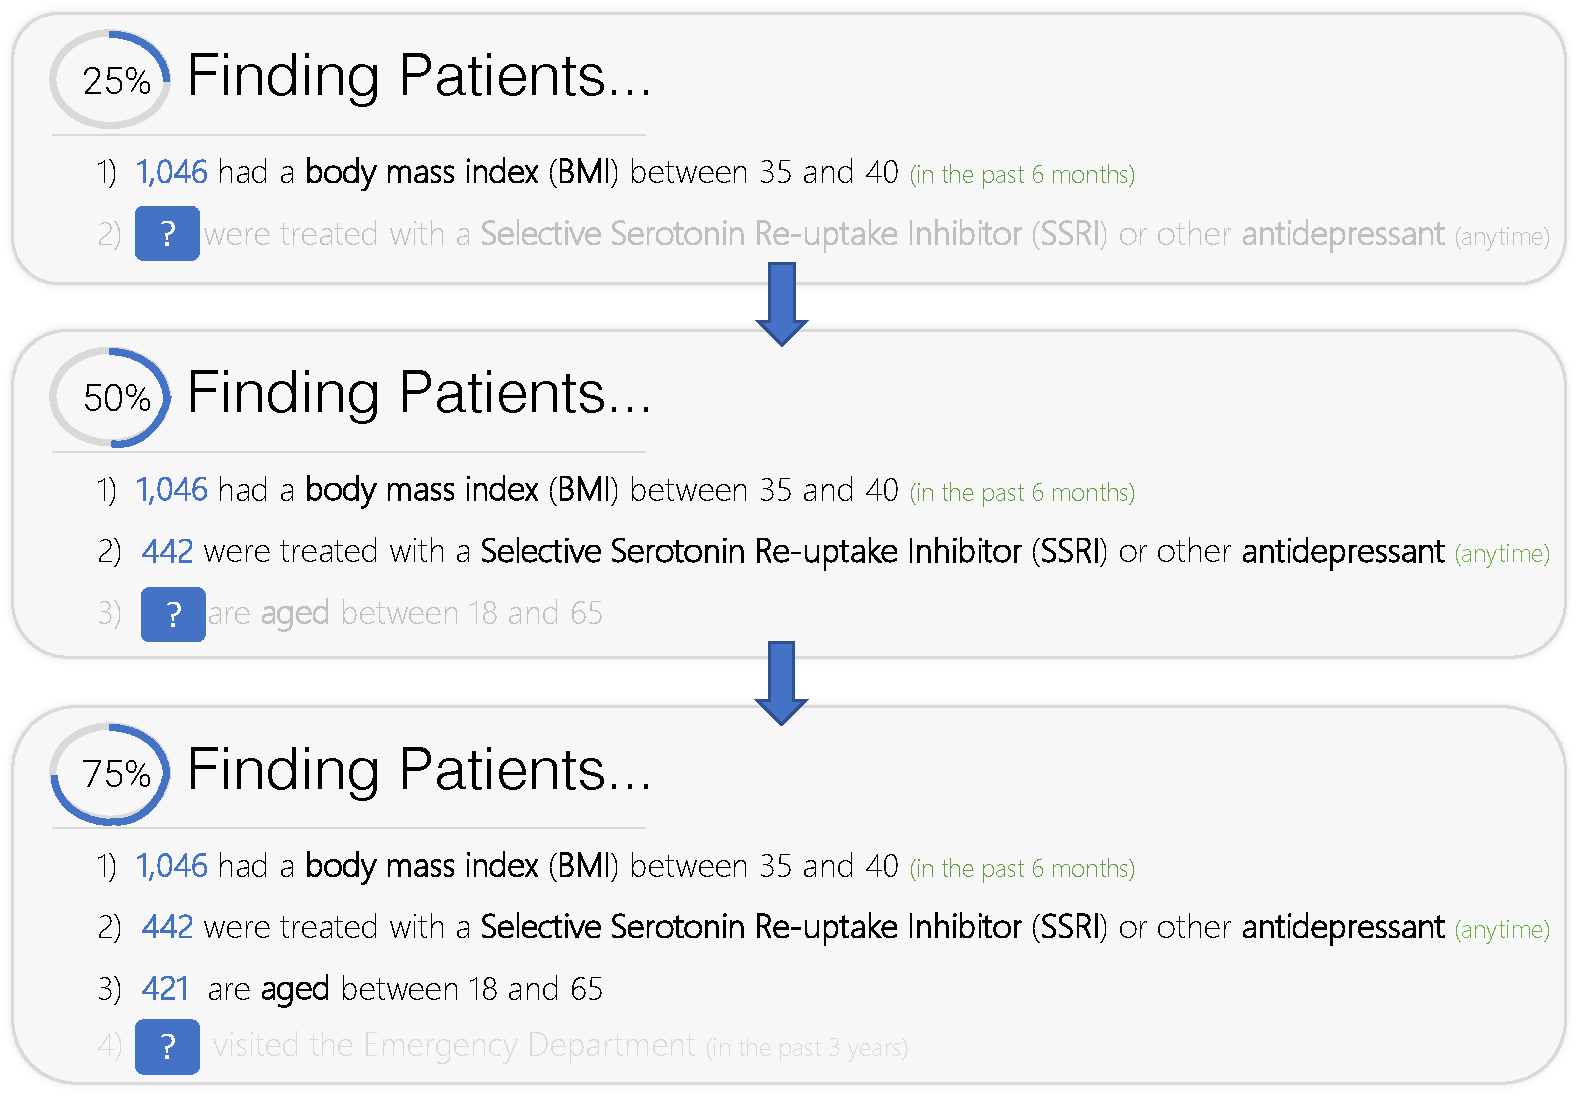
\includegraphics[scale=0.5]{Figures/Aim3/aim3_query_progress.pdf}  
  \caption{}
\label{aim3_fig_query_progress}
\end{figure}

\subsubsection{Evaluation Metrics}

\subsubsection{Limitations}

\end{document}